\section{Hard-coded Approach}

The tasks of "Hard-code Approach" involves mainly about defining various states for the robot, giving parameters empirically for each state, and trying to grab Cylinder anywhere on the table.In this case the evolutionary algorithm does not need to consider how to optimize the order of the various states and the duration of each state but only needs to optimize the motion parameters in each state. So that it can get a relatively better effect in a shorter time.

\subsection{State Machine}

Such as the picture shown in \autoref{fig:statemachine} there are 5 states in state mashine, and they communicate with 2 control interface: Arm Control and Hand Control.These states: Approach, Prepare, Throw give Arm Control commands(string typ) via ROS, and states: Grasp, Release give Hand Control. In these two Control Interfase , each instruction corresponds to parameters for the control of robot.These parameters were originally obtained empirically and then optimized by evolutionary algorithms later. 

The state of Throw and Release was originally designed to execute Release state after Throw state has been executed for a short time, in order to get a farther throw distance.But because of the bug of model, this will break the entire simulation.So these two states can only be executed at the some time. 

\begin{figure}[tpb]
\centering
	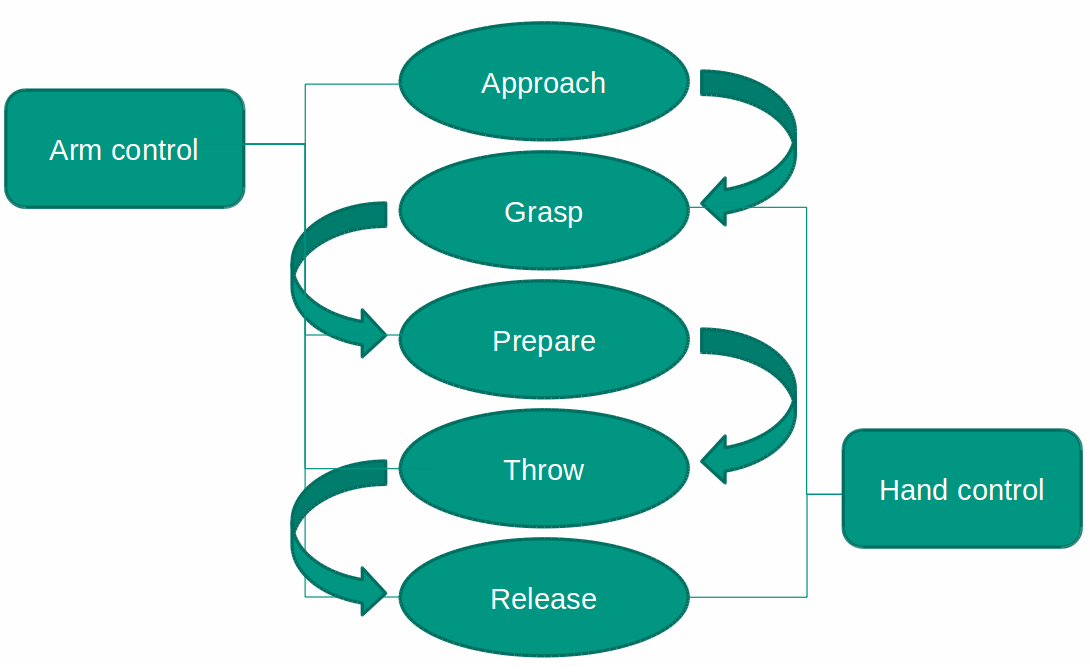
\includegraphics[width=0.96\linewidth]{figures/state.png} 
	\caption{State and Control Interface}
	\vspace{-0.4cm}
	\label{fig:statemachine}
\end{figure}

\subsection{Inverse Kinematics}

The ability to grab a cylinder anywhere on the table is achieved by inverse Kinematic. Because the camera in the model cannot get the depth value of the object, its coordinates are not available through the camera. So as a simplification, when the cylinder is generated, its world coordinates are immediately posted to a topic. As the picture shown in \autoref{fig:top},we assume that the cylinder posion ist $(C_x, C_y, C_z)$, and the robitic origin position is  $(R_x, R_y, R_z)$, so the amr0 move configution $M_0$ can be caculate with the equation below:


\begin{equation}
\label{simple_equation}
M_0=\alpha = arctan((C_y-R_y)/(C_x-R_x))
\end{equation}









\begin{figure}[htpb]
\centering
	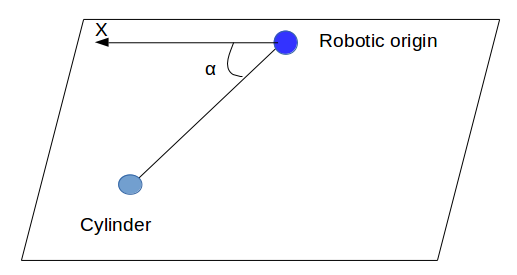
\includegraphics[width=0.96\linewidth]{figures/top_view.png} 
	\caption{Platform top view}
	\vspace{-0.4cm}
	\label{fig:top}
\end{figure}


The \autoref{fig:right} show the look of the model from the right side. Since there is already a perfect configution that makes the robot close to the cylinder(that means $\beta$ and $\gamma$ is known).So the lengs of arm1: a and arm4: b can be caculated with:

\begin{equation}
\begin{aligned}
a=c*sin(\gamma)/sin(\delta)\\b=c*sin(\beta)/sin(\delta)\\ 
\textbf{with}\ c=\sqrt{(R_x-C_x)^2+(R_y-C_y)^2}\\\delta=2*\pi-\beta-\gamma.
\end{aligned}
\end{equation}



When the cylinder is created anywhere on the table, the move configuration of arm1:$M_1$ amr4: $M_4$, arm6: $M_6$ can be caculate with equation below since amr1 and arm4 lengs are known.The move configutions for arm3, amr5 remain the same as before. 
 


\begin{equation}
\begin{aligned}
M_1=\beta=arccos((a^2+c^2-b^2)/2*a*c)\\
M_4=\pi-\delta=\pi-arccos((a^2+b^2-c^2)/2*a*b)\\
M_6=\gamma=arccos((b^2+c^2-a^2)/2*b*c)\\
\textbf{with}\ c=\sqrt{(R_x-C_x)^2+(R_y-C_y)^2}
\end{aligned}
\end{equation}

\begin{figure}[tpb]
\centering
	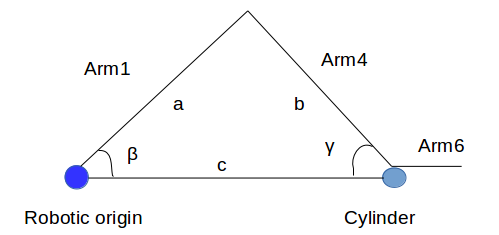
\includegraphics[width=0.96\linewidth]{figures/right_view.png} 
	\caption{Platform right view}
	\vspace{-0.4cm}
	\label{fig:right}
\end{figure}



